%**************************************************************************
%*
%*  Paper: ``INSTRUCTIONS FOR AUTHORS OF LATEX DOCUMENTS''
%*  Publication: 2026 Winter Simulation Conference Author Kit
%*
%*  Filename: wsc26paper.tex
%*
%*  Date: January 14, 2026
%*
%*  Word Processing System: TeXstudio
%*
%**************************************************************************


\documentclass{wscpaperproc}
\usepackage{latexsym}
%\usepackage{caption}
\usepackage{graphicx}
\usepackage{mathptmx}
\usepackage[T1]{fontenc}


%
%****************************************************************************
% AUTHOR: You may want to use some of these packages. (Optional)
\usepackage{amsmath}
\usepackage{amsfonts}
\usepackage{amssymb}
\usepackage{amsbsy}
\usepackage{amsthm}
%****************************************************************************


%
%****************************************************************************
% AUTHOR: If you do not wish to use hyperlinks, then just comment
% out the hyperref usepackage commands below.

%% This version of the command is used if you use pdflatex. In this case you
%% cannot use ps or eps files for graphics, but pdf, jpeg, png etc are fine.

\usepackage[pdftex,colorlinks=true,urlcolor=blue,citecolor=black,anchorcolor=black,linkcolor=black]{hyperref}

%% The next versions of the hyperref command are used if you adopt the
%% outdated latex-dvips-ps2pdf route in generating your pdf file. In
%% this case you can use ps or eps files for graphics, but not pdf, jpeg, png etc.
%% However, the final pdf file should embed all fonts required which means that you have to use file
%% formats which can embed fonts. Please note that the final PDF file will not be generated on your computer!
%% If you are using WinEdt or PCTeX, then use the following. If you are using
%% Y&Y TeX then replace "dvips" with "dvipsone"

%%\usepackage[dvips,colorlinks=true,urlcolor=blue,citecolor=black,%
%% anchorcolor=black,linkcolor=black]{hyperref}
%****************************************************************************


%
%****************************************************************************
%*
%* AUTHOR: YOUR CALL!  Document-specific macros can come here.
%*
%****************************************************************************

% If you use theoremes
\newtheoremstyle{wsc}% hnamei
{3pt}% hSpace abovei
{3pt}% hSpace belowi
{}% hBody fonti
{}% hIndent amounti1
{\bf}% hTheorem head fontbf
{}% hPunctuation after theorem headi
{.5em}% hSpace after theorem headi2
{}% hTheorem head spec (can be left empty, meaning `normal')i

\theoremstyle{wsc}
\newtheorem{theorem}{Theorem}
\renewcommand{\thetheorem}{\arabic{theorem}}
\newtheorem{corollary}[theorem]{Corollary}
\renewcommand{\thecorollary}{\arabic{corollary}}
\newtheorem{definition}{Definition}
\renewcommand{\thedefinition}{\arabic{definition}}

%%% TREATMENT OF FIGURES -----------------------------------------------------------------------------
    % Alter some LaTeX defaults for better treatment of figures:
    % See p.105 of "TeX Unbound" for suggested values.
    % See pp. 199-200 of Lamport's "LaTeX" book for details.
    %   General parameters, for ALL pages:
    \renewcommand{\topfraction}{0.9}     % max fraction of floats at top
    \renewcommand{\bottomfraction}{0.8}             % max fraction of floats at bottom
    %   Parameters for TEXT pages (not float pages):
    \setcounter{topnumber}{2}
    \setcounter{bottomnumber}{2}
    \setcounter{totalnumber}{4}     % 2 may work better
    \renewcommand{\textfraction}{0.05}  % allow minimal text w. figs
    %   Parameters for FLOAT pages (not text pages):
    \renewcommand{\floatpagefraction}{0.85}      % require fuller float pages
                % N.B.: floatpagefraction MUST be less than topfraction !!
    \renewcommand{\dblfloatpagefraction}{0.85} % require fuller float pages

%#########################################################
%*
%*  The Document.
%*
\begin{document}

%***************************************************************************
% AUTHOR: AUTHOR NAMES GO HERE
% FORMAT AUTHORS NAMES Like: Author1, Author2 and Author3 (last names)
%
%		You need to change the author listing below!
%               Please list ALL authors using last name only, separate by a comma except
%               for the last author, separate with "and"
%
\WSCpagesetup{Escudero, Gil-Costa, and Marín}

% AUTHOR: Enter the title, all letters in upper case
\title{DYNAMIC URBAN HEAT EXPOSURE MODELING: A TRAJECTORY-BASED AGENT SIMULATION APPROACH FOR  VULNERABLE POPULATION}
%\title{A TRAJECTORY-BASED AGENT SIMULATION FRAMEWORK FOR URBAN HEAT EXPOSURE ASSESSMENT}

% AUTHOR: Enter the authors of the article, see end of the example document for further examples
\author{\begin{center}
Matías Escudero Bell\textsuperscript{1}, Veronica Gil-Costa\textsuperscript{2}, Mauricio Marin \textsuperscript{1}\\
[11pt]
\textsuperscript{1}Dept.~of Computer Science Engineering, Universidad de Santiago de Chile, Santiago, CHILE\\
\textsuperscript{2}Facultad de Cs. Físico Matemáticas y Naturales, Universidad Nacional de San Luis, San Luis, ARGENTINA\\
\end{center}
}

\maketitle

\vspace{-12pt}

\section*{ABSTRACT}

Heatwave exposure in urban environments is commonly assessed using static spatial indicators, overlooking the dynamic nature of human mobility. This study proposes a trajectory-based agent simulation framework to model heat exposure as a path-dependent process. 
The approach integrates environmental conditions, represented by satellite-derived Normalized Difference Vegetation Index (NDVI), with pedestrian mobility over an urban network. The agents representing older adults traverse the urban network, accumulating heat load as a function of traveled distance and route-level environmental conditions.


The framework is applied to the district of Peñalolén, of the city of Santiago (Chile), enabling the analysis of exposure patterns at the census block level. Results indicate that exposure is primarily driven by travel distance, while vegetation plays a weaker but consistent role in regulating exposure.

Comparison between traditional static indicators based on residential location and the trajectory-based exposure estimates proposed in this study shows that, in our case study,  static approaches tend to overestimate exposure. This underscores the limitations of neglecting mobility and highlights the value of modeling exposure as a trajectory-dependent process

\section{INTRODUCTION}
\label{sec:intro}

Climate change has become one of the most critical challenges of the 21st century, intensifying the frequency, duration, and severity of extreme weather events worldwide \cite{moore2024precipitation}. Among these, heatwaves have emerged as a major concern due to their increasing occurrence and their significant impacts on human health, urban systems, and infrastructure \cite{luber2008heat}. 
Extreme heat events have been linked to substantial increases in mortality and morbidit, particularly in urban environments where local conditions amplify thermal exposure \cite{barriopedro2023heatwaves}. In this context, heatwaves are increasingly recognized as a critical risk factor for urban planning and climate risk management.

The impacts of heatwaves are not evenly distributed across the population, but are strongly conditioned by sociodemographic and environmental factors \cite{wilhelmi2010framework}. In urban contexts, exposure to extreme heat is shaped by the spatial distribution of resources such as vegetation, infrastructure, and access to services, which often reflect underlying socioeconomic inequalities \cite{schwaab2021urban}. Among the most vulnerable groups, older adults are particularly at risk due to physiological sensitivity, higher prevalence of chronic conditions, and limited adaptive capacity \cite{arsad2022heatwaves}. As a result, heat exposure in cities emerges as a complex phenomenon where individual vulnerability interacts with the built environment, amplifying risks in already disadvantaged areas.

%Despite these advances, most existing approaches to heat risk assessment rely on static spatial representations of exposure, typically based on residential location or aggregated spatial units \cite{buscail2012heatwave}.
Despite these advances, most existing approaches to urban heat risk assessment rely on static spatial representations of exposure — typically anchored to residential location or aggregated spatial units — which implicitly assume that individuals remain continuously exposed to the environmental conditions of their place of residence \cite{buscail2012heatwave}. This assumption is particularly problematic for older adults, whose daily mobility, though limited in range, exposes them to diverse microclimatic conditions across the urban environment. Additionally, these approaches commonly use indicators such as land surface temperature or vegetation indices (e.g.,  Normalized Difference Vegetation Index - NDVI) to characterize environmental conditions, providing valuable but inherently static approximations of heat exposure \cite{niu2021heat}. However, such approaches overlook a critical dimension of human experience: individuals are not continuously exposed to the conditions of their place of residence, but rather move across the city throughout the day. As a result, exposure to heat is not fixed in space, but dynamically shaped by mobility patterns and the environmental conditions encountered along daily trajectories. Ignoring this dynamic component may lead to misrepresentation of actual exposure, particularly in urban environments characterized by strong spatial heterogeneity.

Addressing this limitation requires a shift from static representations of heat exposure toward approaches that explicitly account for human mobility and its interaction with the urban environment. In this context, exposure can be understood as a dynamic and path-dependent process, emerging from the interplay between individual characteristics, movement patterns, and spatially heterogeneous environmental conditions. This perspective emphasizes that the risks associated with extreme heat are not only determined by where individuals live, but also by where they travel and the conditions they encounter along their routes. Simulation-based approaches \cite{batty2005cities} \cite{miller2007complex}, particularly those incorporating agent-based representations, offer a suitable framework to capture these interactions, enabling the integration of individual movement, spatial constraints, and environmental variability within a unified modeling structure.

In this study, we propose a geospatial simulation framework that models heat exposure as a dynamic,  cumulative, path-dependent process shaped by individual movement through spatially heterogeneous urban environments. The approach integrates sociodemographic vulnerability derived from census data and environmental conditions represented through satellite-derived vegetation indices (NDVI). Within this framework, agents representing older adults are simulated moving across an urban pedestrian network, where exposure is accumulated along their trajectories as a function of traveled distance and route-level environmental conditions. Rather than reproducing detailed behavioral patterns, the model focuses on generating plausible pedestrian trajectories to estimate cumulative exposure under heterogeneous urban conditions.

The proposed framework is applied to the district of Peñalolén in the city of Santiago, Chile, an urban area characterized by significant socioeconomic and environmental heterogeneity. This case study enables the analysis of fine-scale spatial patterns of heat exposure, showing how exposure is shaped by both residential conditions and movement through the urban environment. 
Results show that travel distance is the primary driver of heat load accumulation, while vegetation cover along routes acts as a consistent but secondary moderating factor. Importantly, static residential-based indicators systematically overestimate exposure compared to trajectory-based estimates, as they fail to account for the environmental variability encountered during movement. These results underscore the value of incorporating mobility into urban heat exposure assessments.

%Results indicate that exposure is not solely determined by place of residence, but is influenced by spatial accessibility and environmental conditions encountered along daily trajectories. In particular, the trajectory-based approach refines exposure estimates by accounting for how individuals move through heterogeneous environments, highlighting differences that are not fully captured by static residential indicators. This perspective contributes to a more nuanced representation of heat exposure and supports improved assessment of urban climate-related risks.

\section{CASE STUDY}
\label{sec:data}

\subsection{City Peñalolén}

We evaluate our proposed framework  using Peñalolén, a district in southeastern Santiago, Chile, as a case study.
 Santiago has been widely characterized by pronounced socio-spatial differentiation, historically shaped by processes of residential segregation and more recent transformations in urban structure \cite{mendez2018inequalities}. These transformations have led to increasingly complex spatial configurations, where traditional patterns of segregation coexist with emerging forms of spatial proximity between different socioeconomic groups \cite{borsdorf2016gated}.

Peñalolén represents a particularly relevant case study within this context. The district has undergone rapid urban expansion and significant demographic change in recent decades, driven in part by the influx of higher-income populations into areas traditionally occupied by lower-income groups. This process has resulted in the spatial coexistence and physical proximity of populations with contrasting socioeconomic characteristics within a relatively compact urban area \cite{villar2021penalolen}.

These dynamics have contributed to the development of a fragmented urban structure, characterized by heterogeneous patterns of land use, infrastructure, and access to urban resources. As a result, Peñalolén provides an appropriate setting to analyze how spatial inequalities are expressed within the urban environment and how they may influence exposure to environmental risks. 
%In particular, the coexistence of diverse socioeconomic groups and contrasting urban morphologies makes it especially suitable for examining how vulnerability, mobility, and environmental conditions interact across space.
In particular, three characteristics make Peñalolén especially suitable for the proposed framework: (i) strong intra-urban environmental heterogeneity, expressed through contrasting vegetation cover across census blocks; (ii) pronounced socioeconomic differentiation spatially associated with environmental conditions; and (iii) a fragmented urban morphology that generates diverse pedestrian accessibility patterns across the district.

\subsection{Vulnerability Data (Census)}

Sociodemographic vulnerability was obtained from the 2024 Chilean census at  the census block level (the smallest available spatial unit). A total of 1,629 census blocks were analyzed within the study area, enabling the identification of fine-scale intra-urban variability.

We calculate the vulnerability  index which aims to capture population characteristics associated with increased sensitivity to extreme heat and reduced adaptive capacity. Based on available census indicators, a set of variables was selected to represent demographic, socioeconomic, and housing-related dimensions of vulnerability. Table~\ref{tab:vulnerability_variables} summarizes the variables included in this work and their interpretation.

\begin{table}[ht]
\caption{Variables used to calculate the heat vulnerability index at the census block level.}
\centering
\begin{tabular}{p{5cm} p{8cm}}
\hline
\textbf{Variable} & \textbf{Interpretation} \\
\hline
Older adult population (\%) & Higher physiological sensitivity to extreme heat events. \\
Illiterate population (\%) & Lower access to information and reduced ability to respond to heat warnings. \\
Overcrowded households (\%) & Increased indoor thermal stress and limited capacity for heat mitigation. \\
Population with tertiary education (\%) & Protective factor associated with higher adaptive capacity. \\
\hline
\end{tabular}
\label{tab:vulnerability_variables}
\end{table}

All variables were standardized using z-scores to ensure comparability across different scales. The proportion of population with tertiary education was incorporated as a protective factor by assigning it a negative contribution in the index. The Heat Vulnerability Index (HVI) for each census block was computed as the arithmetic mean of the standardized variables:

\[
HVI_j = \frac{1}{n} \sum_{k=1}^{n} Z_{jk}
\]

where \(Z_{jk}\) represents the standardized value of variable \(k\) in census block \(j\), and \(n\) is the number of variables included in the index.

To facilitate interpretation and spatial analysis, the resulting index was classified into quintiles, defining five relative levels of vulnerability ranging from very low to very high. This classification enables the identification of spatial patterns of vulnerability and provides a basis for linking sociodemographic conditions with simulated exposure patterns.

The  HVI follows a composite indicator approach commonly used in heat vulnerability assessments \cite{sharma2025heat}, where variable selection and aggregation are adapted to the specific context and data availability. 
%Equal weighting is adopted as a parsimonious assumption in the absence of strong prior evidence supporting differential weights.
Equal weighting is adopted as a transparent and replicable assumption, consistent with common practice in composite vulnerability indices when local empirical evidence supporting differential weighting is unavailable \cite{sharma2025heat}. Sensitivity to this assumption is acknowledged as a limitation of the index construction.

\subsection{Environmental Data (NDVI)}

To characterize the spatial distribution of urban vegetation, a Normalized Difference Vegetation Index (NDVI) raster derived from satellite imagery was incorporated into the analysis. NDVI was computed using Google Earth Engine and used as an indicator of vegetation presence and a proxy for potential mitigation of outdoor thermal exposure.

Vegetation conditions were summarized for each census block using aggregated statistics. Census blocks were aligned to the coordinate reference system of the NDVI raster, and summary statistics were extracted for each polygon. The mean NDVI value was retained as the primary indicator of vegetation availability, while additional statistics (median and maximum) were stored for exploratory analysis.
To facilitate integration into the simulation model, block-level mean NDVI values were normalized to a 0--1 range based on observed minimum and maximum values. This normalized indicator was used as an environmental input in the exposure model.

In addition, NDVI values were intersected with simulated trajectories to estimate route-level vegetation conditions. For each trajectory, NDVI was computed as a length-weighted average of vegetation values across the intersected census blocks, allowing exposure to reflect the environmental conditions experienced along the path rather than only at the origin.

\subsection{Urban Amenities}

To support the generation of spatially consistent pedestrian trajectories, a set of urban amenities was incorporated as potential destinations within the simulation framework. These amenities represent common activity locations within the urban environment and act as spatial anchors for movement across the pedestrian network.

Three categories of amenities were considered: healthcare facilities, commercial establishments, and green areas. These categories were selected as representative of typical daily activities among older adults, including access to services, basic goods, and recreational spaces.

Rather than modeling detailed destination choice behavior, agents are assigned to nearby destinations based on a probabilistic selection process. For each agent, a subset of the nearest destinations is identified, and one destination is selected with probability inversely proportional to distance. This formulation prioritizes spatially accessible locations while preserving stochastic variability in movement patterns.

This approach enables the simulation to capture how exposure accumulates along realistic routes while maintaining a parsimonious modeling structure. The resulting amenity layer provides a simplified representation of urban functions, supporting the analysis of how accessibility and environmental conditions jointly shape heat exposure across the study area.


\section{TRAJECTORY-BASED MODELING FRAMEWORK}
\label{sec:methodology}

%\subsection{Model Overview}

The proposed framework (see Figure \ref{fig:model_overview}) models heat exposure as a dynamic and path-dependent process using a geospatial simulation approach. The model represents individual agents moving across a pedestrian network and accumulating thermal exposure along their trajectories as a function of travel distance and environmental conditions.

The simulation integrates three main components: (i) a spatial representation of the urban environment, including census blocks, vegetation conditions, and urban amenities; (ii) a synthetic population of agents derived from census data; and (iii) a network-based routing mechanism that generates pedestrian trajectories between origins and destinations.

Each agent is initialized within a census block and assigned a representative spatial location. From this location, the agent is connected to the nearest node of the pedestrian network. A destination is then assigned from nearby urban amenities, and a route is computed using shortest-path algorithms based on network distance. This results in a trajectory representing movement across the urban environment.

Heat exposure is accumulated along the route as a function of traveled distance and route-level environmental conditions derived from NDVI. In this formulation, exposure is not treated as a static attribute of location, but as a cumulative process emerging from movement through heterogeneous urban space.

The model adopts a deliberately simplified structure, prioritizing spatial consistency and interpretability over behavioral realism. It does not aim to reproduce detailed decision-making processes, temporal scheduling, or adaptive responses to heat. Instead, it focuses on generating plausible pedestrian trajectories within a realistic urban network to estimate cumulative exposure under spatially heterogeneous conditions. This design choice reflects the framework's primary objective: to demonstrate the added value of mobility-based exposure estimation relative to static residential indicators.

%The model adopts a parsimonious structure and does not aim to reproduce detailed behavioral decision-making. Instead, it focuses on generating spatially consistent trajectories to estimate cumulative exposure under realistic spatial constraints.

\begin{figure}[ht]
    \centering
    \includegraphics[width=0.8\linewidth]{model_overview.png}
    \caption{Conceptual framework of the proposed trajectory-based heat exposure model.}
    \label{fig:model_overview}
\end{figure}

\subsection{Agent Representation}

Agents  represent individuals belonging to the older adult population, identified using census data at the census block level. We select older adult due to its increased sensitivity to extreme heat and its relevance in urban climate risk assessments.
The number of agents assigned to each census block is proportional to the population aged 60 and above, using a scaling factor to construct a synthetic population while maintaining computational tractability. This approach preserves the spatial distribution of vulnerable populations across the study area.

Each agent is characterized by a set of attributes obtained from the census dataset, including its associated census block, a vulnerability indicator, and local environmental conditions such as vegetation levels. In addition, each agent has a representative spatial location within its corresponding census block, which serves as the origin point for trajectory generation.

To enable network-based routing, each agent is linked to the nearest node in the pedestrian network, ensuring that all simulated movements occur within the spatial structure of the urban network.

\subsection{Trajectory Generation}

For each agent, a destination is assigned from a set of urban amenities, including healthcare facilities, commercial establishments, and green areas. Possible destinations are first filtered based on proximity, selecting a subset of the nearest locations.

From this subset of possible destinations, one destination is selected probabilistically, with selection weights inversely proportional to distance. This formulation prioritizes spatially accessible destinations while preserving stochastic variability in destination choice.

Once a destination is assigned, a route between origin and destination is computed using a shortest-path algorithm over the pedestrian network, where edge weights correspond to segment length.

This process generates trajectories that follow the structure of the urban network and reflect spatial accessibility constraints. The resulting trajectories are used to estimate cumulative heat exposure along movement across the district.


\subsection{Thermal Exposure Model}

Thermal exposure is modeled as a cumulative process along each agent's trajectory within the pedestrian network. For a given route, exposure is defined as a function of the total distance traveled and the environmental conditions encountered along the path.

Vegetation is incorporated as a proxy for heat mitigation using NDVI-derived indicators. For each simulated trajectory, a route-level NDVI value is computed by intersecting the route geometry with census blocks and averaging local vegetation conditions weighted by the length of the trajectory within each block. This allows the model to capture spatial variability in environmental conditions along the route. %When route-level NDVI cannot be computed, the NDVI value of the origin census block is used as a fallback.
To integrate vegetation into the exposure calculation, NDVI values are normalized to a 0--1 range based on the observed minimum and maximum values across census blocks. Heat exposure is then defined as:

\[
\text{HeatLoad}_i = L_i \cdot \max\left(r_{\min},\; r_0 - \beta \cdot NDVI_i^{*}\right)
\]

where \(L_i\) is the total length of the trajectory for agent \(i\), \(NDVI_i^{*}\) is the normalized mean NDVI along the route, \(r_0\) is the baseline exposure rate, \(\beta\) represents the cooling strength of vegetation, and \(r_{\min}\) is a lower bound preventing unrealistically low exposure values. 
In this study, parameters are set to \(r_0 = 1.0\), \(\beta = 0.5\), and \(r_{\min} = 0.2\). The baseline rate \(r_0 \) is set to unity for normalization purposes. The cooling coefficient \(\beta\) was selected to reflect a moderate vegetation effect on thermal exposure, consistent with the role of urban greenery as a partial rather than complete heat mitigator \cite{schwaab2021urban}. The lower bound \(r_{\min} = 0.2\) prevents unrealistically low exposure values in densely vegetated areas where full mitigation is physiologically implausible. 


Exposure increases proportionally with travel distance, while vegetation reduces the effective exposure rate along the trajectory. Given the multiplicative structure of the metric, route length is expected to be the dominant component of heat load, with NDVI acting as a moderating factor.

This approach captures heat exposure as a cumulative effect of movement through heterogeneous environmental conditions, rather than as a static attribute of location. By incorporating both distance and route-level vegetation, the model reflects how exposure emerges from the interaction between urban form and individual movement.

\subsection{Simulation Setup}

The simulation framework was implemented in Python, integrating geospatial data processing and network analysis libraries. Spatial data handling was performed using GeoPandas, while routing operations were conducted on a pedestrian network extracted from OpenStreetMap and processed using NetworkX and OSMnx.

Vegetation data was obtained from satellite imagery and processed using Google Earth Engine (GEE), from which NDVI rasters were generated and subsequently integrated into the Python workflow. Block-level statistics were computed to associate NDVI values with census blocks, and route-level vegetation exposure was estimated through spatial intersection and length-weighted averaging along the simulated trajectories.

Each simulation run consists of generating a synthetic population of agents distributed across census blocks, assigning destinations from nearby urban amenities, and computing trajectories over the pedestrian network using shortest-path routing. Destination selection incorporates a stochastic component, where agents choose among nearby locations with probabilities inversely related to distance.
Thermal exposure is then calculated for each trajectory as a function of traveled distance and route-level environmental conditions. %, following the formulation described in the thermal exposure model.


\section{RESULTS}

\subsection{Baseline Spatial Patterns}

Figure~\ref{fig:ndvi_vuln} presents the spatial distribution of vegetation conditions (NDVI) and the Heat Vulnerability Index (HVI) across the study area. Both variables exhibit marked intra-urban heterogeneity, revealing contrasting spatial configurations across different sectors of the district.

Higher NDVI values correspond to areas with greater vegetation cover. In contrast, lower NDVI values are observed in more densely built-up sectors. The vulnerability index shows an inverse configuration, with higher vulnerability levels concentrated in areas characterized by lower vegetation availability.

%To facilitate interpretation, both NDVI and the vulnerability index were classified into quintiles, allowing a consistent comparison of relative spatial gradients across variables. This representation highlights the spatial coexistence of lower vegetation availability and higher vulnerability in several sectors of the study area.

%The relationship between vegetation and vulnerability is further illustrated in Figure~\ref{fig:ndvi_scatter}, which shows a strong negative correlation between NDVI and the vulnerability index ($r = -0.64$). This pattern suggests that census blocks with lower vegetation availability also tend to exhibit higher vulnerability levels.


The relationship between vegetation and vulnerability is further illustrated in Figure~\ref{fig:ndvi_scatter}, which reveals a strong negative correlation between NDVI and the vulnerability index ($r = -0.64$). This spatial co-occurrence has direct implications for the simulation: agents residing in high-vulnerability census blocks are systematically more likely to depart from and travel through areas with lower vegetation cover, compounding their thermal exposure relative to agents in lower-vulnerability areas.

These baseline patterns indicate that environmental and sociodemographic conditions are spatially associated within the study area. This initial spatial structure provides the context for the trajectory-based simulation of mobility and heat exposure examined in the following sections.

\begin{figure}
    \centering
    \includegraphics[width=0.7\linewidth]{vuln_ndvi_maps.png}
    \caption{Spatial distribution of (a) NDVI and (b) Heat Vulnerability Index at the census block level.}
    \label{fig:ndvi_vuln}
\end{figure}

\begin{figure}
    \centering
    \includegraphics[width=0.5\linewidth]{scatter_ndvi_vuln.png}
    \caption{Relationship between NDVI and the Heat Vulnerability Index at the census block level.}
    \label{fig:ndvi_scatter}
\end{figure}

\subsection{Simulated Trajectories}

The simulation generated individual pedestrian trajectories across the urban network based on the spatial distribution of agents and the assignment of nearby destination points. 


A total of 1,862 trips were initially simulated. After applying a maximum walking distance threshold of 1,200 meters, 1,649 trips remained (approximately 88.6\% of all simulated trips). The 213 excluded trips exceeded this threshold and were predominantly associated with census blocks located in peripheral areas of the district, where the spatial separation between residential origins and the nearest available amenities is larger. This exclusion criterion reflects a physiologically plausible upper bound for pedestrian travel among older adults and is consistent with established walkability thresholds in the literature.

%A total of 1,862 trips were initially simulated, of which 1,649 were retained after applying a maximum walking distance threshold of 1,200 meters, corresponding to approximately 88.6\% of all simulated trips.

The resulting trajectories are characterized by relatively short travel distances, with a mean distance of approximately 460 meters and a median of around 410 meters. Most simulated trips are  shorter than the imposed threshold, indicating predominantly local movement patterns
This pattern is consistent with the structure of the model, where destinations are selected from a subset of nearby amenities and assigned with probabilities inversely related to distance. As a result, agents are more likely to travel to spatially accessible locations, leading to a distribution of trajectories dominated by local movements.

Additionally, the configuration of the pedestrian network and the spatial distribution of origins and destinations further constrain route lengths, reinforcing the prevalence of short-distance trajectories.  Overall, the simulated trajectories reflect localized movement patterns shaped by proximity-based destination assignment and network structure, providing the basis for estimating cumulative heat exposure along routes.

\subsection{Simulated Heat Exposure}

%Heat exposure was quantified for each simulated trajectory using the cumulative heat load metric, which integrates traveled distance and route-level environmental conditions. Results show a strong positive relationship between route length and heat load ($r = 0.91$), indicating that distance is the dominant component of exposure under the adopted formulation.This result is consistent with the multiplicative structure of the heat load metric, where exposure increases proportionally with distance, while environmental conditions act as a moderating factor.

Heat exposure was quantified for each simulated trajectory using the cumulative heat load metric, which integrates traveled distance and route-level environmental conditions. Results show a strong positive Pearson correlation between route length and heat load ($r = 0.91$), computed across all simulated trajectories, indicating that distance is the dominant component of exposure under the adopted formulation.

This result is consistent with the multiplicative structure of the heat load metric, where exposure increases proportionally with distance, while environmental conditions act as a moderating factor.

In addition to distance, vegetation conditions along the route also influence exposure levels. A negative Pearson correlation is observed between route-level NDVI and heat load ($r = -0.19$), indicating that trajectories passing through areas with higher vegetation tend to experience lower effective exposure. Although this effect is weaker than that of distance, it consistently contributes to reducing exposure along trajectories.

To assess the added value of the trajectory-based approach, simulated exposure was compared with a static baseline derived from residential vegetation conditions. Static exposure was defined as an inverse function of normalized NDVI at the origin location, representing exposure as a fixed attribute of place of residence.

Both static and dynamic exposure measures were normalized to a common 0--1 scale. Figure~\ref{fig:static_dynamic_scatter} shows the relationship between both measures. 
While a positive association is observed between static and dynamic exposure, the substantial dispersion around the regression line (Figure~\ref{fig:static_dynamic_scatter}) reveals that individuals sharing similar residential environmental conditions can experience markedly different heat loads depending on their destination choice and the vegetation conditions encountered along their specific routes. This within-group variability is a key finding: it demonstrates that residential indicators, even when accurate on average, fail to capture meaningful individual-level differences in exposure that only emerge when mobility is explicitly modeled.

%While a positive association is observed, substantial dispersion indicates that individuals with similar residential conditions may experience different exposure levels depending on their movement patterns.

%Figure~\ref{fig:delta_distribution} presents the distribution of differences between dynamic and static exposure. Results show a consistent tendency toward lower exposure values under the trajectory-based formulation. This pattern suggests that static indicators may overestimate exposure relative to mobility-based estimates under the present modeling assumptions.


Figure~\ref{fig:delta_distribution}  shows the distribution of differences between trajectory-based (dynamic) and residential-based (static) exposure estimates, computed for each simulated trajectory as the difference between both measures (dynamic minus static), after normalizing them to a common scale. The $x$-axis represents the difference in exposure values, while the $y$-axis indicates the frequency of trajectories within each difference interval. Negative values correspond to cases where trajectory-based exposure is lower than static exposure, whereas positive values indicate the opposite.

The distribution is skewed toward negative values, indicating that, for most trajectories, the exposure estimated using the trajectory-based approach is lower than that obtained from static residential indicators. This pattern suggests that static measures tend to overestimate exposure under the present modeling assumptions, as they do not account for variability in environmental conditions encountered along individual movement paths.
\begin{figure}
    \centering
    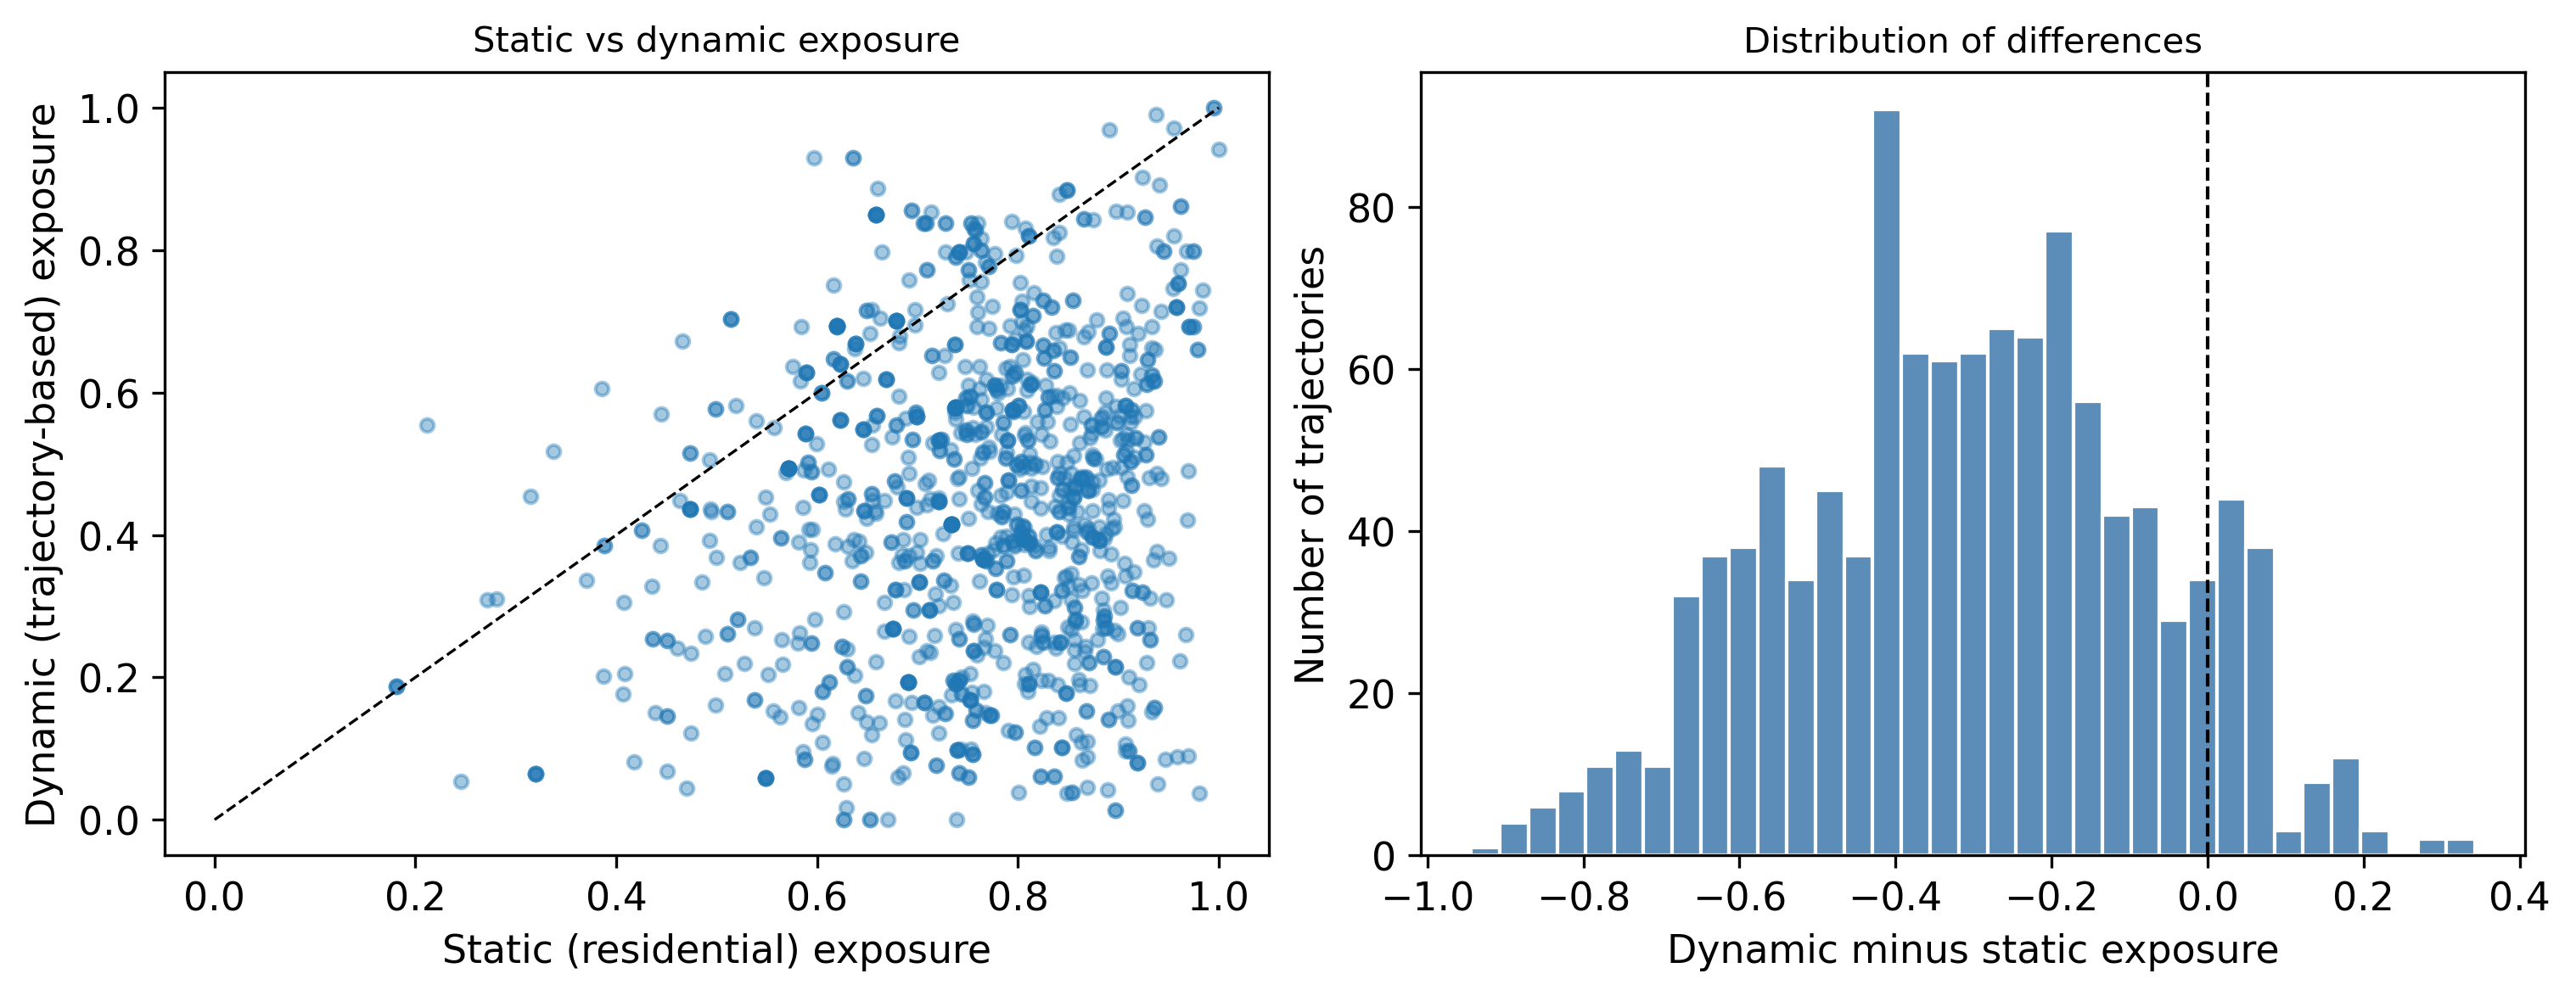
\includegraphics[width=0.5\linewidth]{scatter_static_dynamic.png}
    \caption{Relationship between static (residential) and dynamic (trajectory-based) exposure.}
    \label{fig:static_dynamic_scatter}
\end{figure}

\begin{figure}
    \centering
    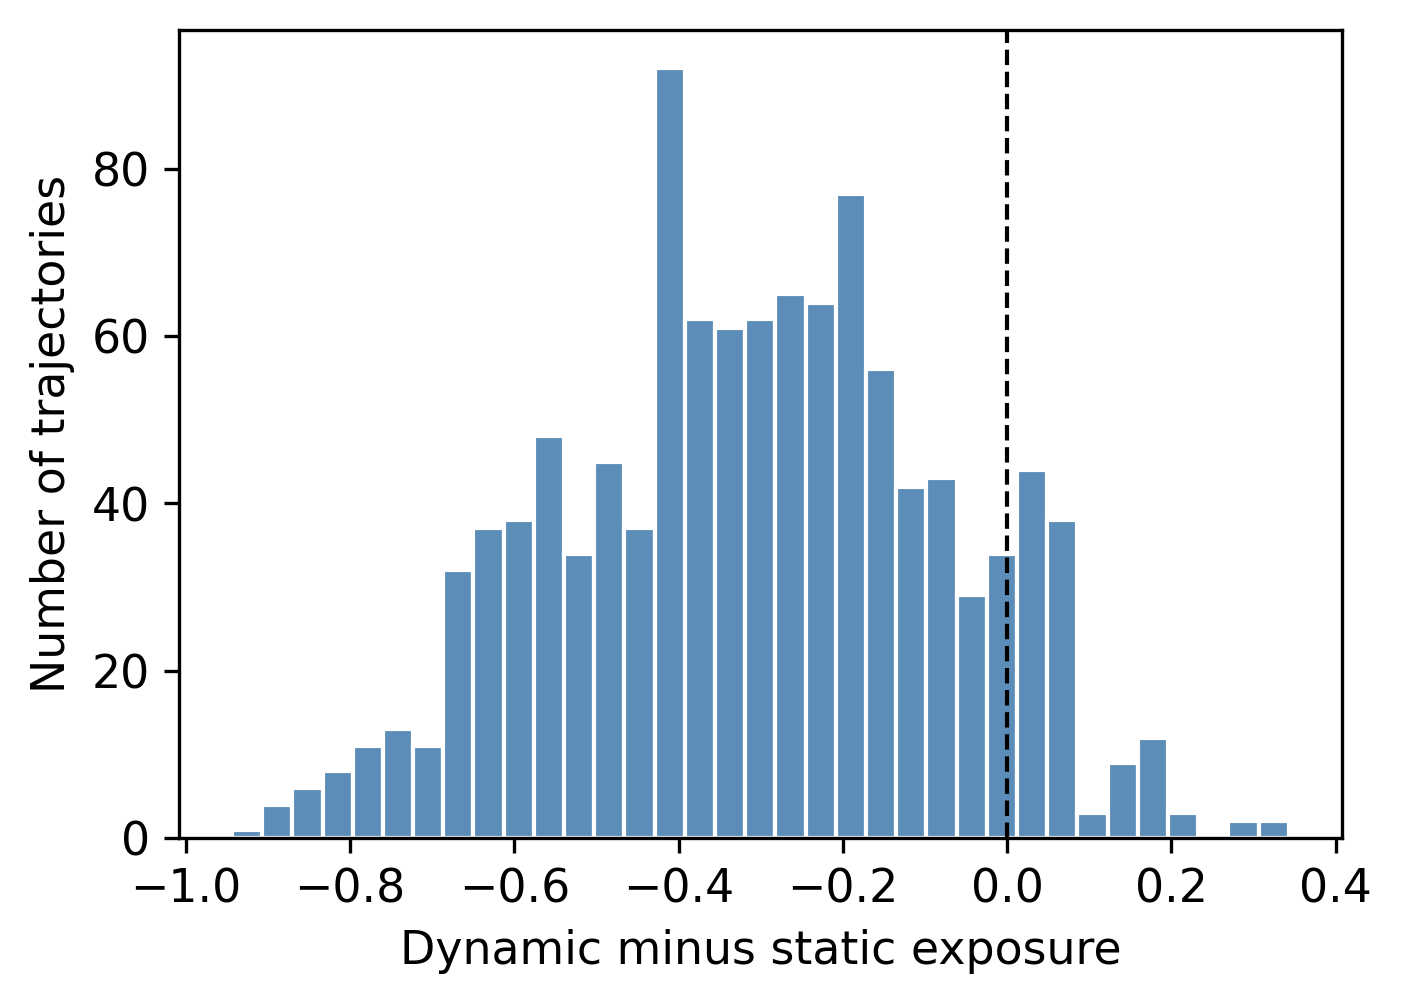
\includegraphics[width=0.45\linewidth]{delta_boxplot.png}
    \caption{Distribution of differences between dynamic and static exposure.}
    \label{fig:delta_distribution}
\end{figure}


\subsection{Heat Exposure Across Vulnerability Groups}

%Differences in heat exposure were observed across vulnerability groups, revealing systematic variations in the simulated outcomes. On average, agents belonging to higher vulnerability groups exhibited higher heat loads compared to those in lower vulnerability categories.

Differences in heat exposure were observed across vulnerability groups (Figure \ref{fig:boxplot_heat}). Agents in the high-vulnerability group showed a higher median heat load compared to those in the low-vulnerability group, with the difference driven by two compounding mechanisms: (i) their residential locations are associated with lower vegetation cover, increasing the effective exposure rate per unit of distance traveled; and (ii) the spatial distribution of amenities relative to high-vulnerability census blocks tends to produce slightly longer routes on average. %However, the overlap between group distributions is substantial, indicating that vulnerability group alone is not a strong predictor of individual heat load. A formal comparison of group means, including effect size estimation, is warranted in future work to assess the statistical robustness of these differences."
This pattern is consistent with the underlying spatial configuration of the study area, where higher vulnerability levels tend to co-occur with lower vegetation availability. %As a result, agents located in more vulnerable areas are more likely to experience environmental conditions associated with higher exposure.
%In addition, differences in travel distances across agents contribute to variation in exposure levels, reinforcing disparities across vulnerability groups. Given the structure of the model, these differences reflect the combined effect of spatial distribution of vulnerability, environmental conditions, and mobility patterns.

These results indicate that heat exposure is unevenly distributed across the population and is shaped by the interaction between sociodemographic characteristics and the spatial configuration of the urban environment. Rather than being determined solely by place of residence, exposure emerges from the joint influence of location and movement across heterogeneous urban conditions.

\begin{figure}
    \centering
    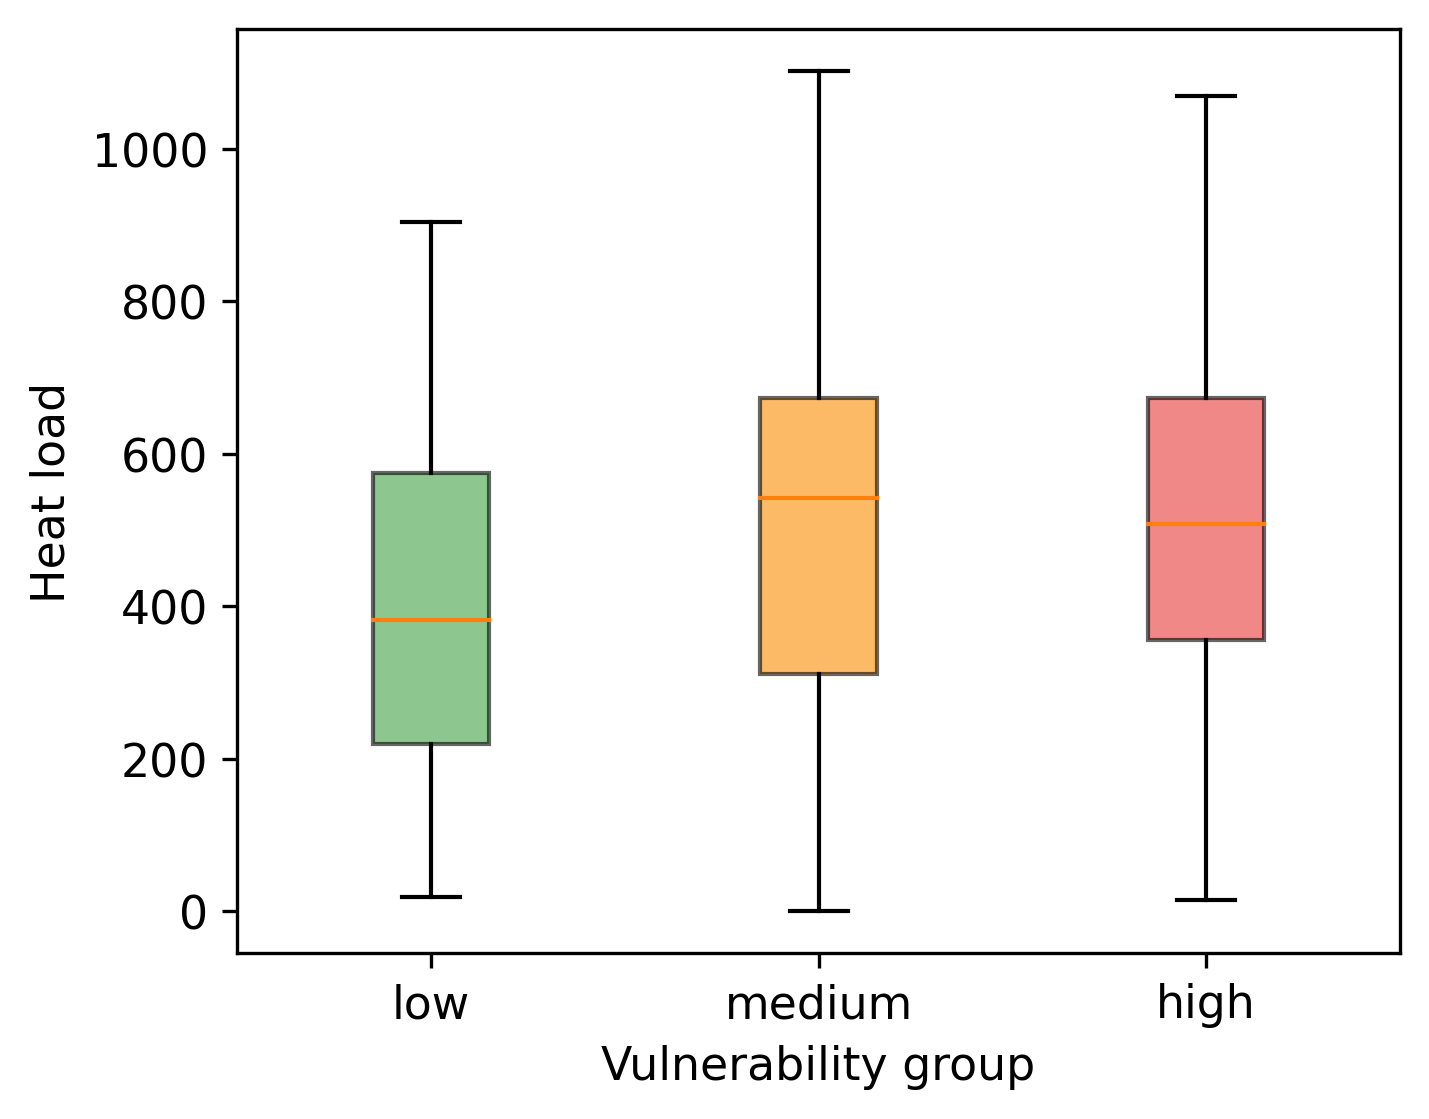
\includegraphics[width=0.5\linewidth]{inequality_boxplot.png}
    \caption{Distribution of heat load across vulnerability groups.}
    \label{fig:boxplot_heat}
\end{figure}

\section{DISCUSSION}

\subsection{Dynamic Nature of Heat Exposure}

The results highlight the importance of modeling heat exposure as a dynamic, trajectory-based process rather than as a static condition associated solely with place of residence. While traditional approaches typically assess exposure based on environmental conditions at fixed locations, the proposed framework shows that exposure can be conceptualized as emerging from the interaction between individual mobility and spatial heterogeneity.

By simulating pedestrian trajectories, the model captures how exposure accumulates along movement paths, revealing patterns that are not represented by static spatial indicators alone. Within this formulation, distance traveled plays a central role in shaping exposure levels, acting as the primary mechanism through which heat load is accumulated. At the same time, environmental conditions encountered along the route, such as vegetation cover, act as a moderating factor.

The comparison between static and dynamic exposure provides an additional insight into how exposure is represented. Results indicate that, under the present formulation, static measures tend to yield higher exposure values than trajectory-based estimates. This difference arises because static approaches implicitly assume constant exposure conditions at the place of residence, while the trajectory-based model accounts for movement through spatially heterogeneous environments.

Rather than fundamentally altering the overall spatial structure of exposure, the dynamic model refines it by incorporating mobility and route-level environmental variability. In particular, the results suggest that shorter travel distances and variation in environmental conditions along trajectories contribute to reducing effective exposure relative to residential-based approximations.

From a planning perspective, these findings suggest that relying exclusively on residential indicators may lead to incomplete representations of exposure intensity. While static measures remain useful for identifying broad spatial patterns, incorporating mobility provides a more nuanced characterization of how exposure is experienced within urban environments.

\subsection{Implications for Inequality and Urban Planning}

The observed differences across vulnerability groups are consistent with the underlying spatial configuration of the study area, where higher vulnerability levels tend to co-occur with lower vegetation availability. As a result, agents associated with more vulnerable areas tend to experience higher exposure levels within the simulation framework.

At the same time, the results indicate that mobility contributes to shaping these differences by introducing variation in both travel distances and environmental conditions encountered along trajectories. This highlights that exposure is not solely determined by residential location, but by the interaction between spatial context and movement.

In practical terms, the proposed approach can inform targeted heat mitigation strategies in at least two ways. First, by identifying route corridors with high pedestrian traffic and low vegetation cover in high-vulnerability areas, urban planners can prioritize street tree planting or shading infrastructure where it would have the greatest impact on reducing cumulative exposure. Second, by revealing mismatches between residential vulnerability and actual trajectory-based exposure, the framework can help redirect heat-health interventions toward populations whose real exposure differs substantially from what residential indicators would suggest.

\subsection{Limitations and Future Work}

Several limitations of the proposed framework should be explicitly acknowledged. First, the heat exposure metric relies on a simplified proxy combining travel distance and vegetation-derived cooling, without incorporating ambient temperature data, time-of-day variation, or physiological heat strain models. As a result, the metric captures relative differences in exposure across agents rather than absolute thermal load values. Second, agent behavior follows a single-trip, shortest-path structure that omits temporal scheduling, multi-stop itineraries, and adaptive responses to environmental conditions. In practice, older adults may make multiple trips per day, substantially increasing cumulative exposure beyond what the current model captures.
Third, the results are inherently dependent on the structure and assumptions of the model, including destination assignment rules and the formulation of the heat exposure metric. As such, the findings should be interpreted as model-based insights rather than direct measurements of real-world exposure.

As future work we plan to extend the framework by incorporating time-dependent environmental data, more detailed behavioral representations, and validation against empirical mobility or health data. These extensions would allow for a more comprehensive assessment of heat exposure dynamics and their implications for urban risk management.

\section{CONCLUSION}

This study proposed a geospatial simulation framework to model heat exposure as a trajectory-based process, integrating pedestrian mobility, urban network structure, and environmental conditions derived from satellite data. By representing exposure as a cumulative process along movement paths, the approach extends traditional static assessments based on residential location.

The results indicate that heat exposure is strongly influenced by travel distance, while environmental conditions such as vegetation cover play a weaker but consistent role in modulating exposure levels. The comparison between static and dynamic measures shows that, under the present formulation, residential-based indicators tend to yield higher exposure values than trajectory-based estimates, as they do not account for variability introduced by mobility.

Rather than fundamentally altering the overall spatial distribution of exposure, the trajectory-based approach refines its representation by incorporating movement and route-level environmental variability. This highlights the importance of considering mobility when assessing exposure, particularly in urban contexts characterized by short-distance travel and heterogeneous environmental conditions.

Overall, the proposed framework contributes to improving the representation of urban heat exposure by linking static environmental indicators with mobility-driven processes. While the model relies on a simplified proxy of exposure, it provides a flexible and interpretable approach for capturing how exposure emerges from the interaction between spatial structure and individual movement.

%Future work could extend this framework by incorporating temporal variability in environmental conditions, alternative mobility modes, and more detailed behavioral representations, as well as exploring validation against empirical mobility or health data to further assess its applicability in urban climate risk analysis.


% Reducing font size (to 9pt) for References & Author Biagraphies
\footnotesize

% Please don't exchange the bibliographystyle style
\bibliographystyle{wsc}

% AUTHOR: Include your bib file here
\bibliography{demobib}


\section*{AUTHOR BIOGRAPHIES}

\noindent {\bf \MakeUppercase{Matías Escudero Bell}} is a doctoral student in Engineering Sciences with a major in Computer Science at Universidad de Santiago de Chile. His research focuses on geospatial data science, urban analytics, and simulation-based modeling for environmental risk assessment. His work integrates spatial data, agent-based modeling, and optimization techniques to support decision-making in urban and environmental contexts. His email address is \email{matias.escudero.b@usach.cl}.\\

\noindent {\bf \MakeUppercase{Veronica Gil-Costa}} is a full professor  at Universidad Nacional de San Luis, Argentina. Her research interests include modeling and simulation, agent-based systems, and complex systems analysis. She has extensive experience in computational modeling applied to socio-technical and environmental systems. Her email address is \email{gvcosta@unsl.edu.ar}.\\

\noindent {\bf \MakeUppercase{Mauricio Marin }} is a former researcher at Yahoo! Labs Santiago hosted by the University of Chile, and currently a
full professor at University of Santiago, Chile.  His research work is on parallel computing and distributed systems with applications in query
processing and capacity planning for Web search engines. His email address is \email{mauricio.marin@usach.cl}.

\end{document}

